% ============================================================
%  CS-404 BDA  ·  Assignment 2  ·  NUST SEECS  ·  2026
%  Compile with:  xelatex profiling_report.tex  (run twice)
% ============================================================
\documentclass[12pt, a4paper]{article}

% ── Font (Aptos — requires XeLaTeX) ─────────────────────────
\usepackage{fontspec}
\setmainfont{Aptos}
\setsansfont{Aptos}

% ── Page Layout ─────────────────────────────────────────────
\usepackage[top=2.5cm, bottom=2.5cm, left=2.8cm, right=2.8cm]{geometry}
\usepackage{setspace}
\usepackage{parskip}
\setstretch{1.25}
\setlength{\parskip}{5pt}

% ── Colors ──────────────────────────────────────────────────
\usepackage{xcolor}
\definecolor{primary}{RGB}{0, 83, 150}
\definecolor{rowgray}{RGB}{245, 247, 250}
\definecolor{phred}{RGB}{190, 20, 20}

% ── Tables ──────────────────────────────────────────────────
\usepackage{booktabs}
\usepackage{longtable}
\usepackage{array}
\usepackage{colortbl}
\newcolumntype{L}[1]{>{\raggedright\arraybackslash}p{#1}}
\newcolumntype{C}[1]{>{\centering\arraybackslash}p{#1}}

% ── Figures ─────────────────────────────────────────────────
\usepackage{graphicx}
\usepackage{float}
\usepackage{caption}
\captionsetup{font=small, labelfont=bf, skip=5pt}

% ── Section Headings ────────────────────────────────────────
\usepackage{titlesec}
\titleformat{\section}
  {\large\bfseries\color{primary}}{\thesection.}{0.5em}{}
  [\vspace{1pt}{\color{primary!35}\rule{\linewidth}{0.6pt}}]
\titleformat{\subsection}
  {\normalsize\bfseries}{\thesubsection.}{0.5em}{}
\titleformat{\subsubsection}
  {\small\bfseries}{\thesubsubsection.}{0.4em}{}
\titlespacing{\section}{0pt}{14pt}{6pt}
\titlespacing{\subsection}{0pt}{10pt}{4pt}

% ── Header / Footer ─────────────────────────────────────────
\usepackage{fancyhdr}
\pagestyle{fancy}
\fancyhf{}
\lhead{\small\color{primary} CS-404 BDA · Assignment 2}
\rhead{\small\color{primary} NUST SEECS · Spring 2026}
\cfoot{\small\thepage}
\renewcommand{\headrulewidth}{0.3pt}

% ── Hyperlinks ──────────────────────────────────────────────
\usepackage{hyperref}
\hypersetup{colorlinks, linkcolor=primary, urlcolor=primary}

% ── Lists ───────────────────────────────────────────────────
\usepackage{enumitem}
\setlist[itemize]{topsep=2pt, itemsep=1pt, leftmargin=1.4em}
\setlist[enumerate]{topsep=2pt, itemsep=1pt, leftmargin=1.6em}

% ── Placeholder command ─────────────────────────────────────
%  After running the notebook, replace \ph{...} with real values
\newcommand{\ph}[1]{{\color{phred}\textit{[#1]}}}

% ============================================================
\begin{document}

% ─────────────────────────────────────────────────────────────
%  TITLE PAGE
% ─────────────────────────────────────────────────────────────
\begin{titlepage}
\centering
\vspace*{2cm}

{\large\bfseries National University of Sciences \& Technology (NUST)}\\[4pt]
{\normalsize School of Electrical Engineering and Computer Science (SEECS)}\\[2pt]
{\normalsize Department of Computing}

\vspace{1.2cm}
{\color{primary}\rule{0.75\linewidth}{1.2pt}}\\[12pt]
{\huge\bfseries\color{primary} Assignment 2}\\[8pt]
{\LARGE Data Source Selection \& Ingestion Pipeline}\\[12pt]
{\color{primary}\rule{0.75\linewidth}{1.2pt}}

\vspace{0.8cm}
{\large CS-404 Big Data Analytics \quad|\quad Spring 2026}

\vspace{1.4cm}
\begin{tabular}{clc}
\toprule
\textbf{Sr.} & \textbf{Name} & \textbf{Qalam ID} \\
\midrule
1 & Hassan Sufyan        & 468149 \\
2 & Saim Kaleem Arain    & 460353 \\
3 & Muhammad Saad Akhtar & 458102 \\
\bottomrule
\end{tabular}

\vspace{1.2cm}
\renewcommand{\arraystretch}{1.4}
\begin{tabular}{@{}ll}
\textbf{Instructor:} & Ms.\ Zahida Kausar \\
\textbf{Date:}       & 15 April 2026 \\
\textbf{GitHub:}     & \ph{Add URL after pushing repo} \\
\end{tabular}

\vfill
\end{titlepage}

% ─────────────────────────────────────────────────────────────
\tableofcontents
\newpage

% =============================================================
\section{Dataset Selection}
% =============================================================

\subsection{About the Dataset}

\begin{center}
\renewcommand{\arraystretch}{1.3}
\begin{tabular}{@{} L{3.5cm} L{10cm} @{}}
\toprule
\textbf{Property} & \textbf{Details} \\
\midrule
\rowcolor{rowgray}
Name       & UK Road Safety: Traffic Accidents and Vehicles \\
Source     & Kaggle — \texttt{daveianhickey/2000-16-traffic-flow-england-scotland-wales} \\
\rowcolor{rowgray}
Publisher  & UK Department for Transport (\url{https://data.gov.uk}) \\
Coverage   & England, Scotland \& Wales, 2005–2014 \\
\bottomrule
\end{tabular}
\end{center}

\vspace{4pt}
The dataset uses the UK government's \textbf{STATS19} road accident recording scheme.
Four CSV files were downloaded and ingested into HDFS:

\vspace{4pt}
\begin{center}
\renewcommand{\arraystretch}{1.3}
\begin{tabular}{L{5.6cm} r r C{2.8cm}}
\toprule
\textbf{File} & \textbf{Size} & \textbf{Rows} & \textbf{Period} \\
\midrule
\rowcolor{rowgray}
\texttt{accidents\_2005\_to\_2007.csv} & 156 MB & 570,011 & 2005–2007 \\
\texttt{accidents\_2009\_to\_2011.csv} & 129 MB & 469,442 & 2009–2011 \\
\rowcolor{rowgray}
\texttt{accidents\_2012\_to\_2014.csv} & 127 MB & 464,697 & 2012–2014 \\
\texttt{ukTrafficAADF.csv}             &  53 MB & 275,387 & Multi-year \\
\midrule
\textbf{Total} & \textbf{465 MB} & \textbf{1,779,537} & \\
\bottomrule
\end{tabular}
\end{center}

\vspace{4pt}
\textit{Note: The 2008 accident file is absent from this Kaggle version.
With 1.5 million accident records, the dataset is $3\times$ the 500K minimum threshold.}

% ---
\subsection{Warehouse Suitability}

\begin{itemize}
  \item \textbf{Scale.} 1.78M records require distributed storage (HDFS) and processing (Spark).
  \item \textbf{Attribute diversity.} Geographic (lat/lon), temporal (date, time), categorical (severity, weather, road type), and numeric (speed limit, casualty count) columns span all data types.
  \item \textbf{Star schema fit.} The accident event is a natural fact table. Clear dimension candidates include Time, Geography, Road Characteristics, Environmental Conditions, and Traffic Flow.
  \item \textbf{Credible source.} Published by the UK Department for Transport — the same data used for national road safety policy.
\end{itemize}

% ---
\subsection{Business Questions}

\begin{enumerate}[label=\textbf{BQ\arabic*.}]
  \item \textbf{When are roads most dangerous?} — Identify peak risk by hour, day, and month.
  \item \textbf{Which road user type is most vulnerable?} — Compare casualty rates by vehicle/user category.
  \item \textbf{Where do accidents cluster?} — Pinpoint geographic hotspots for infrastructure investment.
  \item \textbf{How does junction type affect accident severity?} — Compare severity at junction vs.\ non-junction sites across junction configurations.
  \item \textbf{Which combination of road type, speed limit, and weather produces the most fatal accidents?} — Multi-dimensional analysis to support evidence-based speed limit policy.
\end{enumerate}


% =============================================================
\section{HDFS Ingestion Pipeline}
% =============================================================

The script \texttt{ingest.py} runs end-to-end without manual intervention across five steps:

\vspace{4pt}
\begin{center}
\renewcommand{\arraystretch}{1.35}
\begin{tabular}{c L{2.5cm} L{9.5cm}}
\toprule
\textbf{Step} & \textbf{Action} & \textbf{Description} \\
\midrule
\rowcolor{rowgray}
1 & Load    & Downloads the dataset from Kaggle using the API (\texttt{KaggleApi}). \\
2 & Validate & Checks each CSV for file size, UTF-8 encoding, and row count. \\
\rowcolor{rowgray}
3 & Organize & Creates a partitioned HDFS directory: \texttt{/warehouse/raw/uk\_road\_safety/year=YYYY/month=MM/} \\
4 & Upload  & Pushes each validated CSV to HDFS via the \texttt{hdfs} Python library. \\
\rowcolor{rowgray}
5 & Log     & Records every step (success/warning/error) to \texttt{ingestion\_pipeline.log}. \\
\bottomrule
\end{tabular}
\end{center}

\vspace{8pt}
Figure~\ref{fig:hdfs} confirms the four files were uploaded with correct paths and sizes.

\begin{figure}[H]
  \centering
  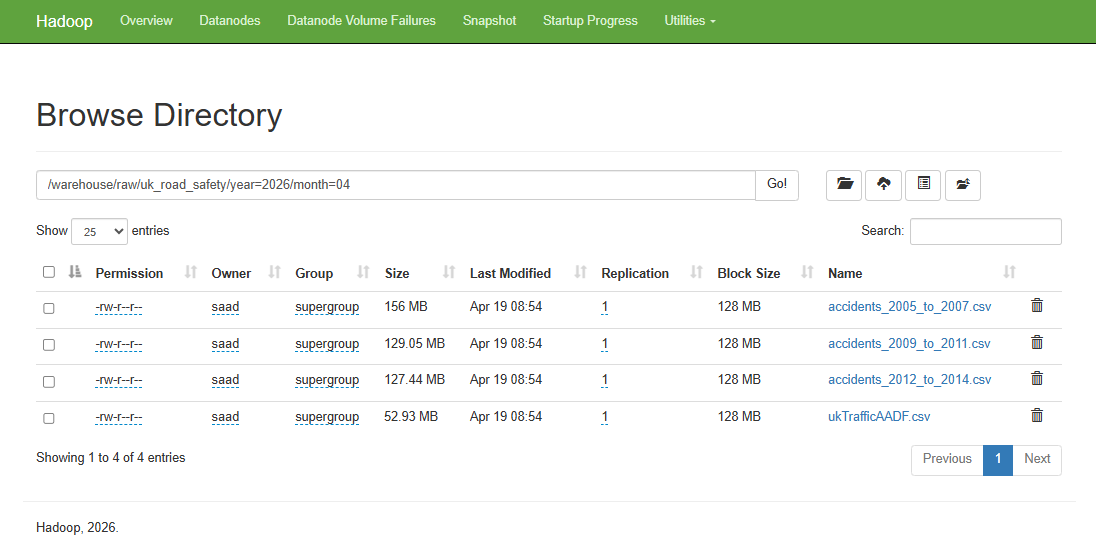
\includegraphics[width=0.92\textwidth]{hdfs_screenshot.png}
  \caption{Hadoop WebUI showing the four uploaded files in \texttt{/warehouse/raw/uk\_road\_safety/year=2026/month=04/}}
  \label{fig:hdfs}
\end{figure}


% =============================================================
\section{Data Profiling Report}
% =============================================================

\textit{All analyses use Python (pandas, matplotlib, seaborn) on the raw CSV files in
\texttt{./raw\_data/}. Run \texttt{profiling\_notebook.ipynb} to generate all figures and
statistics, then replace every \ph{placeholder} below with the printed output.}

% ---
\subsection{Schema Description}

\subsubsection{Accident Dataset — \ph{N} columns · 1,504,150 rows}

\begin{center}
\small
\renewcommand{\arraystretch}{1.3}
\begin{longtable}{L{4.2cm} C{2.2cm} L{4.5cm} L{2.6cm}}
\toprule
\textbf{Column} & \textbf{Type} & \textbf{Description} & \textbf{Sample} \\
\midrule
\endfirsthead
\toprule
\textbf{Column} & \textbf{Type} & \textbf{Description} & \textbf{Sample} \\
\midrule
\endhead
\bottomrule
\endlastfoot

\rowcolor{rowgray}
\texttt{Accident\_Index}      & string  & Unique accident identifier (PK) & \texttt{200501BS00001} \\
\texttt{Longitude}            & float64 & WGS84 longitude                 & \texttt{-0.1727} \\
\rowcolor{rowgray}
\texttt{Latitude}             & float64 & WGS84 latitude                  & \texttt{51.4895} \\
\texttt{Accident\_Severity}   & string  & Fatal / Serious / Slight        & \texttt{Slight} \\
\rowcolor{rowgray}
\texttt{Number\_of\_Vehicles} & int64   & Vehicles involved               & \texttt{2} \\
\texttt{Number\_of\_Casualties}& int64  & Casualties in accident          & \texttt{1} \\
\rowcolor{rowgray}
\texttt{Date}                 & string  & DD/MM/YYYY — needs parsing      & \texttt{04/01/2005} \\
\texttt{Day\_of\_Week}        & string  & Monday – Sunday                 & \texttt{Tuesday} \\
\rowcolor{rowgray}
\texttt{Time}                 & string  & HH:MM (24h) — needs parsing     & \texttt{17:42} \\
\texttt{Road\_Type}           & string  & Single/dual carriageway, etc.   & \texttt{Single carriageway} \\
\rowcolor{rowgray}
\texttt{Speed\_limit}         & int64   & Posted speed limit (mph)        & \texttt{30} \\
\texttt{Junction\_Detail}     & string  & Junction type (null if none)    & \texttt{T or staggered} \\
\rowcolor{rowgray}
\texttt{Junction\_Control}    & string  & Traffic control at junction     & \texttt{Give way} \\
\texttt{Light\_Conditions}    & string  & Daylight / Darkness variants    & \texttt{Daylight} \\
\rowcolor{rowgray}
\texttt{Weather\_Conditions}  & string  & Fine / Rain / Snow / Fog / etc. & \texttt{Fine no high winds} \\
\texttt{Road\_Surface\_Conditions} & string & Dry / Wet / Ice / Snow     & \texttt{Dry} \\
\rowcolor{rowgray}
\texttt{Carriageway\_Hazards} & string  & Oil / Pedestrian / None (many nulls) & \texttt{None} \\
\texttt{Urban\_or\_Rural\_Area} & string & Urban or Rural                 & \texttt{Urban} \\
\rowcolor{rowgray}
\texttt{LSOA\_of\_Accident\_Location} & string & Lower Super Output Area   & \texttt{E01000001} \\
\texttt{Year}                 & int64   & Calendar year                   & \texttt{2005} \\
\end{longtable}
\end{center}

\subsubsection{Traffic Flow Dataset (ukTrafficAADF) — \ph{N} columns · 275,387 rows}

Key columns: \texttt{Count\_point\_id}, \texttt{Year}, \texttt{Region}, \texttt{Road} (e.g.\ A1, M25),
\texttt{RoadCategory}, \texttt{Easting}/\texttt{Northing}, \texttt{AllMotorVehicles},
plus per-class vehicle counts (\texttt{CarsTaxis}, \texttt{AllHGVs}, \texttt{Motorcycles}, etc.).

% ---
\subsection{Missing Value Analysis}

\begin{center}
\small
\renewcommand{\arraystretch}{1.3}
\begin{tabular}{L{5.5cm} r r}
\toprule
\textbf{Column} & \textbf{Missing Count} & \textbf{Missing (\%)} \\
\midrule
\rowcolor{rowgray}
\ph{Column 1 — from notebook Cell 5} & \ph{N} & \ph{\%} \\
\ph{Column 2} & \ph{N} & \ph{\%} \\
\rowcolor{rowgray}
\ph{Column 3} & \ph{N} & \ph{\%} \\
\ph{Column 4} & \ph{N} & \ph{\%} \\
\rowcolor{rowgray}
\ph{...remaining columns with nulls} & \ph{N} & \ph{\%} \\
\bottomrule
\multicolumn{3}{l}{\textit{\small Fill from notebook output after running Cell 5.}}
\end{tabular}
\end{center}

\begin{figure}[H]
  \centering
  \includegraphics[width=0.92\textwidth]{figures/missing_values_bar.png}
  \caption{Missing value percentage per column. Red = $>$20\%, Orange = 5–20\%, Blue = $<$5\%.}
  \label{fig:missing}
\end{figure}

% ---
\subsection{Statistical Summary}

\begin{center}
\small
\renewcommand{\arraystretch}{1.3}
\begin{tabular}{L{4.8cm} r r r r r}
\toprule
\textbf{Column} & \textbf{Mean} & \textbf{Median} & \textbf{Std Dev} & \textbf{Min} & \textbf{Max} \\
\midrule
\rowcolor{rowgray}
\texttt{Number\_of\_Casualties} & \ph{} & \ph{} & \ph{} & \ph{} & \ph{} \\
\texttt{Number\_of\_Vehicles}   & \ph{} & \ph{} & \ph{} & \ph{} & \ph{} \\
\rowcolor{rowgray}
\texttt{Speed\_limit}           & \ph{} & \ph{} & \ph{} & \ph{} & \ph{} \\
\texttt{Longitude}              & \ph{} & \ph{} & \ph{} & \ph{} & \ph{} \\
\rowcolor{rowgray}
\texttt{Latitude}               & \ph{} & \ph{} & \ph{} & \ph{} & \ph{} \\
\texttt{Year}                   & \ph{} & \ph{} & \ph{} & 2005  & 2014  \\
\bottomrule
\multicolumn{6}{l}{\textit{\small Fill from notebook Cell 6.}}
\end{tabular}
\end{center}

% ---
\subsection{Distribution Analysis}

\subsubsection{Accident Severity}

\begin{figure}[H]
  \centering
  \includegraphics[width=0.93\textwidth]{figures/severity_distribution.png}
  \caption{Accident severity — count (left) and proportional breakdown (right).}
\end{figure}

\textbf{Finding:} Most accidents (\ph{\%}) result in \textit{Slight} injury. \textit{Fatal} accidents
are rare (\ph{\%}). This imbalance affects any severity-based model and must be considered
when designing KPIs in the A3 fact table.

\subsubsection{Speed Limit at Accident Site}

\begin{figure}[H]
  \centering
  \includegraphics[width=0.90\textwidth]{figures/speed_limit_dist.png}
  \caption{Speed limit distribution at accident sites (invalid values excluded).}
\end{figure}

\textbf{Finding:} The 30 mph limit dominates, reflecting urban accident concentration.
Secondary peaks at 60 mph (rural A-roads) and 70 mph (motorways) follow the UK road
network composition. Invalid values ($\leq 0$): \ph{N records, \%} — data entry errors.

\subsubsection{Number of Casualties per Accident}

\begin{figure}[H]
  \centering
  \includegraphics[width=0.93\textwidth]{figures/casualties_distribution.png}
  \caption{Casualty histogram (left, capped at 99th percentile) and box plot (right).}
\end{figure}

\textbf{Finding:} Distribution is strongly right-skewed. Median = \ph{} (one casualty per
accident is the norm). Extreme outliers up to \ph{max} casualties are present. Median-based
imputation (not mean) is appropriate for related fields in A3.

\subsubsection{Accident Frequency by Hour of Day}

\begin{figure}[H]
  \centering
  \includegraphics[width=0.93\textwidth]{figures/hourly_accidents.png}
  \caption{Accidents per hour of day. Red bars = rush hours (07–09, 16–18).}
\end{figure}

\textbf{Finding:} Two peaks align with morning and evening commutes. The trough at 02:00–05:00
reflects low traffic volume. The derived \texttt{Hour} column (A3 ETL) will serve as a
Time dimension attribute directly addressing BQ1.

\subsubsection{Accident Frequency by Day of Week}

\begin{figure}[H]
  \centering
  \includegraphics[width=0.90\textwidth]{figures/day_of_week.png}
  \caption{Total accidents by day of week, 2005–2014.}
\end{figure}

\textbf{Finding:} Weekdays have higher accident volume (commuter traffic). Friday records the
highest count. Weekend accidents, though fewer in total, carry a higher proportion of
serious/fatal outcomes — consistent with higher speeds and alcohol-related incidents.

% ---
\subsection{Data Quality Issues}

\begin{center}
\small
\renewcommand{\arraystretch}{1.3}
\begin{tabular}{c L{3.5cm} l r r}
\toprule
\textbf{\#} & \textbf{Column(s)} & \textbf{Issue Type} & \textbf{Count} & \textbf{\%} \\
\midrule
\rowcolor{rowgray}
1 & \texttt{Junction\_Control} & Structural nulls  & \ph{N} & \ph{\%} \\
2 & \texttt{2nd\_Road\_Class/Number} & Structural nulls & \ph{N} & \ph{\%} \\
\rowcolor{rowgray}
3 & \texttt{Speed\_limit} & Invalid values ($\leq$0) & \ph{N} & \ph{\%} \\
4 & \texttt{Date} (all rows) & Wrong type — string not datetime & 1,504,150 & 100\% \\
\rowcolor{rowgray}
5 & \texttt{Time} & Wrong type — HH:MM string & \ph{N} & \ph{\%} \\
6 & \texttt{LSOA\_of\_Accident\_Location} & Missing (older records) & \ph{N} & \ph{\%} \\
\rowcolor{rowgray}
7 & \texttt{Carriageway\_Hazards} & Missing / text placeholders & \ph{N} & \ph{\%} \\
8 & \texttt{Accident\_Index} & Duplicate PKs (if any) & \ph{N} & \ph{\%} \\
\rowcolor{rowgray}
9 & \texttt{Latitude}/\texttt{Longitude} & Out-of-UK-bounds & \ph{N} & \ph{\%} \\
10 & \texttt{Weather\_Conditions} & Semantic duplicates (e.g.\ \textit{Fine no high winds} vs \textit{Fine + high winds}) & \ph{N cols} & — \\
\bottomrule
\multicolumn{5}{l}{\textit{\small Fill counts from notebook Cells 5, 7, 8, 9.}}
\end{tabular}
\end{center}

% ---
\subsection{Proposed Cleaning Strategy}

Each action below is specific and justified.
Vague statements (e.g.\ ``handle missing values'') are intentionally avoided.

\begin{longtable}{c L{3cm} L{5cm} L{4.2cm}}
\toprule
\textbf{\#} & \textbf{Issue} & \textbf{Action in A3 ETL} & \textbf{Justification} \\
\midrule
\endfirsthead
\toprule
\textbf{\#} & \textbf{Issue} & \textbf{Action in A3 ETL} & \textbf{Justification} \\
\midrule
\endhead
\bottomrule
\endlastfoot
\small
\rowcolor{rowgray}
1 &
\texttt{Junction\_Control} — nulls at non-junction sites &
Fill with \texttt{'No Junction Applicable'} &
Null means no junction exists — not unknown. This category enables BQ4 junction analysis. \\

2 &
\texttt{2nd\_Road\_Class / Number} — null when no 2nd road &
String: fill \texttt{'N/A'}. Numeric: fill sentinel \texttt{-1} &
Absence of a second road is structural, not missing data. Sentinel \texttt{-1} is outside valid range and filterable in Spark SQL. \\

\rowcolor{rowgray}
3 &
\texttt{Speed\_limit} $\leq 0$ — data entry errors (\ph{N, \%}) &
Replace with \textbf{median} speed limit grouped by \texttt{Road\_Type} using PySpark \texttt{Window} &
Median is robust to skew. Grouping by road type preserves context (motorway median $\neq$ urban median). \\

4 &
\texttt{Date} — string in all 1.5M rows &
Parse to \texttt{DateType} (\texttt{to\_date(..., 'dd/MM/yyyy')}); derive \texttt{Year}, \texttt{Month}, \texttt{DayOfWeek}, \texttt{Quarter} &
Required for Spark SQL time-range queries and the Time dimension in the star schema. \\

\rowcolor{rowgray}
5 &
\texttt{Time} — HH:MM string &
Extract integer \texttt{Hour} (0–23); retain original column &
Hour enables morning/afternoon/night bucketing (BQ1). Original column is kept for audit. \\

6 &
\texttt{LSOA} — missing for \ph{N} older records &
Keep as null; add boolean flag \texttt{lsoa\_available} &
LSOA codes cannot be reverse-geocoded reliably. Flag enables conditional geo-queries. \\

\rowcolor{rowgray}
7 &
\texttt{Carriageway\_Hazards} — nulls and text placeholders (\textit{Data missing or out of range}) &
Convert all text placeholders to \texttt{NaN}; fill remaining nulls with \texttt{'None'} &
Absence of a hazard equals 'None' in STATS19 context. Text placeholders are not standard nulls and must be standardised first. \\

8 &
Duplicate \texttt{Accident\_Index} (\ph{N}) &
\texttt{dropDuplicates(['Accident\_Index'])}, keep first occurrence &
\texttt{Accident\_Index} is the primary key. Duplicates inflate all count-based KPIs. \\

\rowcolor{rowgray}
9 &
Coordinates outside UK bounding box (\ph{N}) &
Add \texttt{is\_coordinate\_valid} flag; exclude from geo-spatial joins only &
Corrupt coordinates cannot be imputed. Records remain valid for non-spatial analysis. \\

10 &
\texttt{Weather\_Conditions} — semantic duplicates (\textit{Fine no high winds} / \textit{Fine + high winds}) &
Standardise into consolidated categories: \textit{Fine}, \textit{Fine (High Winds)}, \textit{Rain}, etc. &
Semantic duplicates create false category splits that undercount true weather conditions in BQ5. \\

\end{longtable}


% =============================================================
\appendix
\section*{Appendix: Ingestion Log (Extract)}
\addcontentsline{toc}{section}{Appendix: Ingestion Log}
% =============================================================

\small
\begin{verbatim}
2026-04-19 08:53:51  INFO  --- Starting Automated Ingestion Pipeline ---
2026-04-19 08:54:16  INFO  Download and extraction successful.
2026-04-19 08:54:21  INFO  Validation passed: accidents_2005_to_2007.csv  570,011 rows  UTF-8
2026-04-19 08:54:24  INFO  Validation passed: accidents_2009_to_2011.csv  469,442 rows  UTF-8
2026-04-19 08:54:28  INFO  Validation passed: accidents_2012_to_2014.csv  464,697 rows  UTF-8
2026-04-19 08:54:29  INFO  Validation passed: ukTrafficAADF.csv           275,387 rows  UTF-8
2026-04-19 08:54:29  INFO  HDFS dir created: /warehouse/raw/uk_road_safety/year=2026/month=04/
2026-04-19 08:54:30  INFO  Upload successful: accidents_2005_to_2007.csv
2026-04-19 08:54:31  INFO  Upload successful: accidents_2009_to_2011.csv
2026-04-19 08:54:33  INFO  Upload successful: accidents_2012_to_2014.csv
2026-04-19 08:54:34  INFO  Upload successful: ukTrafficAADF.csv
2026-04-19 08:54:34  INFO  --- Ingestion Pipeline Completed Successfully ---
\end{verbatim}

\vfill
{\color{primary!40}\rule{\linewidth}{0.4pt}}
\begin{center}
  \small\color{gray}
  CS-404 BDA · Assignment 2 · NUST SEECS · Spring 2026\\
  Hassan Sufyan · Saim Kaleem Arain · Muhammad Saad Akhtar
\end{center}

\end{document}
